% !Mode\dots ``TeX:UTF-8''
% !TEX root = ../bare_jrnl.tex
\section{Preliminaries} 
\label{sec:pre}
In this section we introduce the definition of \BCNs\ and their algebraic forms, as well as the four existing types of observability. 

$\mathbb{B}$ : the set $\{0,1\}$; $t=0,1,\ldots$ represents the discrete time. 

\subsection{Boolean Control Networks}

A Boolean control network can be defined as a directed graph together with logical equations to describe the updating rules of the nodes' value of the directed graph. The formal definition of \BCN\ is given as follows. 

\begin{definition}[Boolean Control Networks, \cite{Ideker2001A}] A \BCN\ consists of the  topology and the associated updating rules. The topology is captured by a directed graph which consists of input-nodes ($\mathfrak{i}$), state-nodes ($\mathfrak{s}$), output-nodes ($\mathfrak{o}$), and directed edges which connect nodes. 
	\begin{itemize}
	\item Every node in a \BCN\ can take a value from $\{0,1\}$ at a discrete time $t=0, 1, 2,\ldots$ 
	
	\item Every directed edge from a state-node $\mathfrak{s}_i$ (or an input-node $\mathfrak{i}_w$) to a state-node $\mathfrak{s}_j$ means that  $\mathfrak{s}_j(t+1)$ is affected by  $\mathfrak{s}_i(t)$ (or $\mathfrak{i}_w(t)$). 
	
	\item Every directed edge from a state-node $\mathfrak{s}_i$ to an output-node $\mathfrak{o}_j$ means that   $\mathfrak{o}_j(t)$  is affected by   $\mathfrak{s}_i(t)$.  
	\end{itemize}

Assuming that the \BCN\ has $n$ state-nodes, $m$ input-nodes and $q$ output-nodes. Then the updating rules of the \BCN\ can be described as following formulas:
\begin{equation}
\begin{split}
\mathfrak{s}(t+1)=&f(\mathfrak{i}(t),\mathfrak{s}(t))\\
\mathfrak{o}(t)=&h(\mathfrak{s}(t))
\end{split}
\label{equ:1}
\end{equation}
where
\begin{itemize}
	\item $\mathfrak{s}(t)\in \mathbb{B}^n$ is a state which represent the value of all state-nodes at time step $t$; 	
	\item $\mathfrak{i}(t)\in \mathbb{B}^m$ is an input which represent the value of all input-nodes at time step $t$; 	
	\item $\mathfrak{o}(t)\in \mathbb{B}^q$ is an output which represent the value of all output-nodes at time step $t$;  
	\item $f:\mathbb{B}^{n+m}\mapsto \mathbb{B}^n$ and $h:\mathbb{B}^n\mapsto \mathbb{B}^q$ are logical functions that represent the updating rules of the {\em BCN}. 
\end{itemize}
%Where $\mathbb{B}$ : the set $\{0,1\}$; $t=0,1,\ldots$ represents the discrete time. 
 

\end{definition}



In order to better illustrate the definition of BCN, we give an example as follows.

%Note that one can only know that whether a node is affected by another node from the network graph. Different \BCNs\ may have the same structure, in order to determine a \BCN\ uniquely, 

 
 \begin{figure}[thpb]
      \centering
      \framebox{\parbox{3in}{
		\centerline{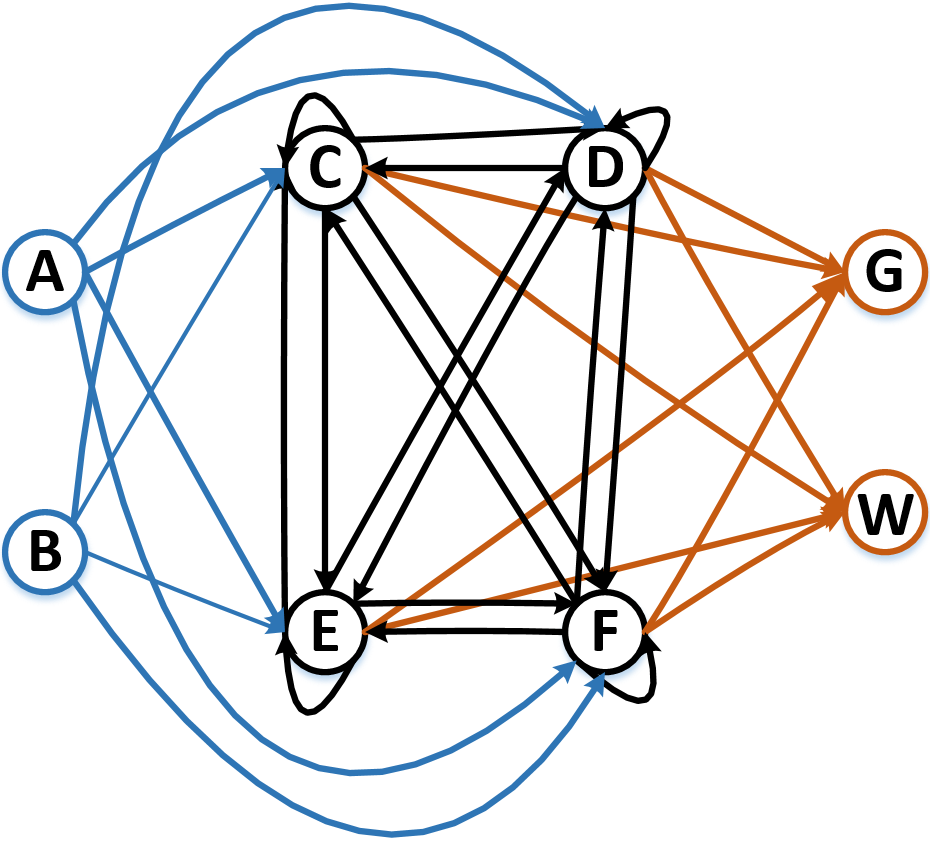
\includegraphics[scale=0.23]{figures/Fig1.png}}
	}}
      
      \caption{A Boolean control network with two input-nodes $A$ and $B$, four state-nodes $C$, $D$, $E$ and $F$, and two output-nodes $G$, $W$. We use blue, black and orange, to distinguish three types of nodes and three types of edges.}
      \label{fig:1}
  \end{figure}

%To better illustrate the concept of {\em BCNs}, we give a simple example to describe it.

\begin{example}
In Fig.\ref{fig:1} we have a \BCN\ with two input-nodes $A$ and $B$, four state-nodes $C$, $D$, $E$ and $F$, two output-nodes $G$, $W$. The node categories  as follows.  
\begin{equation*}
\begin{split}
&A(t), B(t)\in \mathfrak{i}(t),\\
&C(t), D(t), E(t), F(t)\in \mathfrak{s}(t),\\
&G(t), W(t)\in \mathfrak{o}(t)
\end{split}
\label{equ:20}
\end{equation*}
 denote the value of input-nodes, state-nodes, output-nodes at time step $t$, respectively.
The updating rules $f:\mathbb{B}^{6}\mapsto \mathbb{B}^4$ and $h:\mathbb{B}^4\mapsto \mathbb{B}^2$ are shown in the truth table (Fig.\ref{fig:2}).  For instance, the updating rule of output-node $G$ is 
\[G(t)=C(t)\wedge \neg {(\neg {D}(t)\wedge \neg{ E}(t)\wedge \neg{F}(t))}.\]
Without confusion, we short  logical formula $A\wedge B$ as $AB$, and we use $A+B$ to denote logical formula $A\vee B$.  Hence, 
\[G(t)=C(t) \neg {(\neg {D}(t) \neg{ E}(t) \neg{F}(t))}.\]
%\[G(t)=C(t) \neg\left((\neg{D}(t))(\neg{ E}(t))(\neg{F}(t))\right).\]
And the updating rule of state-node $C$ is 

$C(t+1)=(\neg{A}(t)D(t) (\neg{B}(t) \neg{F}(t) (\neg{C}(t) + \neg{E}(t)) + 
C(t)(B(t)E(t)+F(t)))+(A(t)(\neg{D}(t)(\neg{B}(t)\neg{C}(t)+\neg{E}(t)F(t)+
\neg{C}(t)F(t))+B(t)E(t)\neg{F}(t)))+(\neg{B}(t)E(t)(C(t)\neg{D}(t)\neg{F}(t)+
D(t)F(t)))(B(t)\neg{E}(t)(\neg{C}(t)F(t)+C(t)\neg{D}(t))).$

%\[C(t+1)=(A(t)\wedge B(t))\vee (C(t)\wedge D(t))\vee (E(t)\wedge F(t))\]
The reason why we use the truth table to describe the updating rules of the \BCN\ is that it would be more convenient for a \BCN\ to be converted into its aglebraic form. And we will use this example to explain various concepts throughout this paper.
  \begin{figure}[thpb]
      \centering
      \framebox{\parbox{3in}{
		\centerline{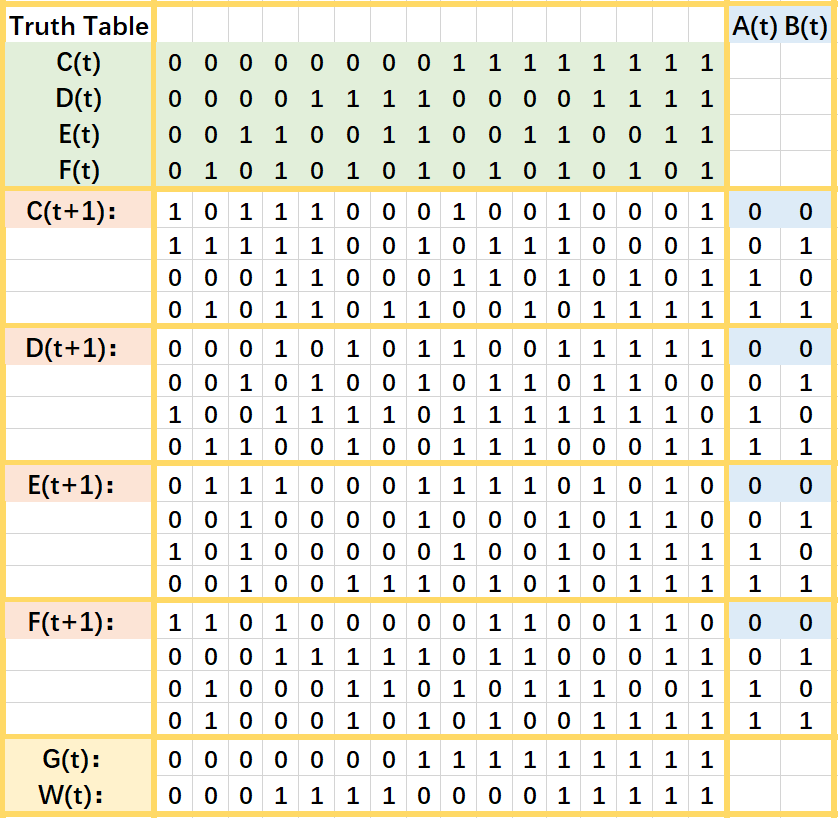
\includegraphics[scale=0.261]{figures/Fig2.png}}
	}}
      
      \caption{The truth table which describe the updating rules of the \BCN\ shown in Fig.\ref{fig:1}.}
      \label{fig:2}
   \end{figure}
   \label{exa:2}
\end{example}   


%==============================================================================================================
\subsection{The algebraic forms of \BCNs}
%\ly{ As mentioned in the {\em Section \ref{sec:intro}}, 
The \emph{semi-tensor product} (\STP) of matrices is one of useful tools to deal with  both \BNs\ and \BCNs\  related problems \cite{cheng2009controllability}. The \STP\ is used to represent the algebraic form of \BCN. With the algebraic form, we can introduce four existing observability of \BCN. The definition of \STP\ is as follows.

\begin{definition}[STP] 
	\cite{Cheng2011Analysis} Let $X\in\mathbb{R}_{m\times n}$, $Y\in\mathbb{R}_{p\times q}$ and $\alpha={\tt lcm}(n,p)$ be the {\em least common multiple} of $n$ and $p$. The \STP\ of $X$ and $Y$ is defined as \[X\ltimes Y=(X\otimes I_{(\frac{\alpha}{n})})(Y\otimes I_{(\frac{\alpha}{p})}),\] where $\otimes$ denotes the {\em Kronecker product}. 
\end{definition}

After introducing the definition of \STP\ of matrices,  we introduce some related notations \cite{Zhang2016Observability}:
\begin{itemize}
  \item $\delta^i_n$: the $i$-th column of the $n\times n $ {\em identity matrix} $I_n$;
  \item $\Delta_n$: the set $\{\delta^1_n,\ldots,\delta^n_n \}$; 
  \item $\delta_n \left[i_1,\ldots,i_s\right]$: $\left[\delta^{i_1}_n,\ldots,\delta^{i_s}_n\right]$ the logical matrix where $i_1,\ldots,i_s\in\left\{1,2,\ldots,n\right\}$;
  \item  $L_{n\times s}$: the set of $n\times s$ logical matrices.
\end{itemize}

Using \STP\ of matrices, the updating rules of the \BCN\ (\ref{equ:1}) can be quivalently represented in the following algebraic form:
\begin{definition}[Algebraic Forms]

\begin{equation}
\begin{split}
\mathsf{s}(t+1)=&\ L\ltimes{\mathsf{i}(t)}\ltimes{\mathsf{s}(t)}\\
\mathsf{o}(t)=&\ H\ltimes{\mathsf{s}(t)}
\end{split}
\label{equ:2}
\end{equation}
where $\mathsf{s}(t)\in\Delta_N$, $\mathsf{i}(t)\in\Delta_M$, and  $\mathsf{o}(t)\in\Delta_Q$ denote the states, inputs and outputs respectively.
% For convenience, we use same notations $\mathsf{s}(t)$, $\mathsf{i}(t)$ and $\mathsf{o}(t)$ in formulas (\ref{equ:1}) and (\ref{equ:2}), but they  are written in different vector forms. 
$L\in L_{N\times\left(NM\right)}$ and $H\in L_{Q\times N}$ denote the relation matrices. $N=2^n$, $M=2^m$, $Q=2^q$ where $n$, $m$ and $q$ represent the number of state-nodes, input-nodes and output-nodes respectively. 
\end{definition}

After the introduction of the algebraic forms of \BCNs, we introduce the process of constructing a \BCN's  algebraic form. In order to construct the algebraic form of \BCN, we give a mapping \[\tau:\{0,1\}\mapsto \{\delta_2^1, \delta_2^2\},\] that $\tau(0)=\delta_2^2$, $\tau(1)= \delta_2^1$. 
%each logical value a vector form as: $1 \scriptsize{\sim} \delta_2^1$, $0 \scriptsize{\sim} \delta_2^2$. 
Therefore, the value of a node takes value from these two vectors, e.g. the input-node $A$ of \BCN\ in {\em Example \ref{exa:2}}, $\tau(A(t))\in \{\delta_2^1, \delta_2^2\}$. Then using the \STP\ of matrices, we have 
\[\mathsf{i}(t)=\mathsf{i}_1(t)\ltimes {\ldots}\ltimes \mathsf{i}_m(t);\] 
\[\mathsf{s}(t)=\mathsf{s}_1(t)\ltimes {\ldots}\ltimes \mathsf{s}_n(t);\] 
\[\mathsf{o}(t)=\mathsf{o}_1(t)\ltimes {\ldots}\ltimes \mathsf{o}_q(t).\] 
For instance, in the {\em Example \ref{exa:2}}, when $C(t+1)=0$, $D(t+1)=1$, $E(t+1)=1$ and $F(t+1)=0$, we have 
\begin{equation*}
\begin{split}
\mathsf{s}(t+1)=&\tau(0) \ltimes \tau(1) \ltimes \tau(1) \ltimes \tau(0)\\
=&\delta_{2}^2 \ltimes \delta_{2}^1 \ltimes \delta_{2}^1 \ltimes \delta_{2}^2\\
=&\delta_{16}^{10}.
\end{split}
\end{equation*}

And according to \cite{Cheng2003Semi}, for the logical function $f_i$ of each state-node $\mathfrak{s}_i$ which can be found in the updating rules ( fomula (\ref{equ:1})) that
\[\mathfrak{s}_i(t+1)=f_i(\mathfrak{i}_1(t),\ldots,\mathfrak{i}_m(t),\mathfrak{s}_1(t),\ldots,\mathfrak{s}_n(t)),\] 
there exists a logical matrix $L_i\in L_{2\times {N M}}$ such that
%\begin{equation}
%\begin{split}
\[\tau(\mathfrak{s}_i(t+1))= L_i\ltimes\mathsf{i}(t)\ltimes\mathsf{s}(t).\]
%\end{split}
%\end{equation}
%where the left side of equation calculate the truth value and the  right side of equation calculate the vector in $\{\delta_2^1, \delta_2^2\}$. 
Therefore for state-nodes $\mathsf{s}_1,\ldots,\mathsf{s}_n$, we have $n$ corresponding logical matrices $L_1,\ldots,L_n$ for them, respectively. 
%We have that
%when\\
If for each state-node $\mathsf{s}_i$ the logical matrix has its form
\[L_i=[\delta_2^{i_1},\ldots,\delta_2^{i_{NM}}],\] 
then we have that %for the set of all state-nodes $s(t)$ the logical matrix 
\[L=[\delta_N^{R_1},\ldots,\delta_N^{R_{NM}}]\]  where 
\[\delta_N^{R_1}=\delta_2^{1_1}\ltimes \ldots \ltimes \delta_2^{n_1};\]\[\vdots\] \[\delta_N^{R_{NM}}=\delta_2^{1_{NM}}\ltimes \ldots \ltimes \delta_2^{n_{NM}}.\] 

%then 

By this relationship we can construct the $L$ for the algebraic forms of \BCNs. And then we can construct the logical matrix $H$ in the similar way. 

%Since \STP\ keeps most properties of the conventional product \cite{Cheng2011Analysis}, the associative law, the distributive law, etc. % We usually omit the symbol ``$\ltimes$'' hereinafter. 

%\ly{For instance, the formula \[\mathsf{s}(t+1)=L\ltimes{\mathsf{i}(t)}\ltimes{\mathsf{s}(t)}\] will be written as  \[\mathsf{s}(t+1)=L{\mathsf{i}(t)}{\mathsf{s}(t)}.\]}


To better illustrate the concept of algebraic forms, we give a simple example to describe it.
\begin{example}
For instance, for the \BCN\ mentioned in {\em Example \ref{exa:2}}, we have that the updating rules of this \BCN\ can be represented with the algebraic form:
\begin{equation*}
\begin{split}
\mathsf{s}(t+1) =&\delta_{16}[\alpha]\ltimes\mathsf{i}(t)\ltimes\mathsf{s}(t)\\
\mathsf{o}(t) =&\delta_4[\beta]\ltimes\mathsf{s}(t)\\
\end{split}
\label{equ:4}
\end{equation*}
where $\alpha=\{10,4,11,16,9,5,1, 7,15,2,3,12,7,6,8,13,8,9,\\15,10,14,4,3,16,1,14,12,13,5,7,2,6,7,2,3,13,13,9,5,1,\\16,13 ,6,14,11,10,4,15,1,14 ,7,6,9 ,8,11,12,5,5,13,3,10,\\12,16,16\}$, $\beta=\{1,1,1,2,2,2,2,3,3,3,3,4,4,4,4,4\}$, $t\in \mathbb{N}$, $\mathsf{s}(t)\in \Delta_{16}$, $\mathsf{i}(t)\in \Delta_4$ and $\mathsf{o}(t)\in \Delta_4$.

And then we have its algebraic form shown by table (Fig.\ref{fig:6}) that $\mathsf{s}(t)\in \Delta_{16}$, $\mathsf{i}(t)\in \Delta_4$ and $\mathsf{o}(t)\in \Delta_4$. For instance, when $\mathsf{s}(t)=\delta_{16}^1$ and  $\mathsf{i}(t)=\delta_{4}^1$, it means that the values of all state-nodes and all input-nodes in time step $t$ are $1$,  from the true table (Fig.\ref{fig:2}) we have $C(t+1)=0$, $D(t+1)=1$, $E(t+1)=1$ and $F(t+1)=0$. Thus we have \[\mathsf{s}(t+1)=\delta_{2}^2 \ltimes \delta_{2}^1 \ltimes \delta_{2}^1 \ltimes \delta_{2}^2=\delta_{16}^{10}.\]
 \begin{figure}[thpb]
      \centering
      \framebox{\parbox{3in}{
		\centerline{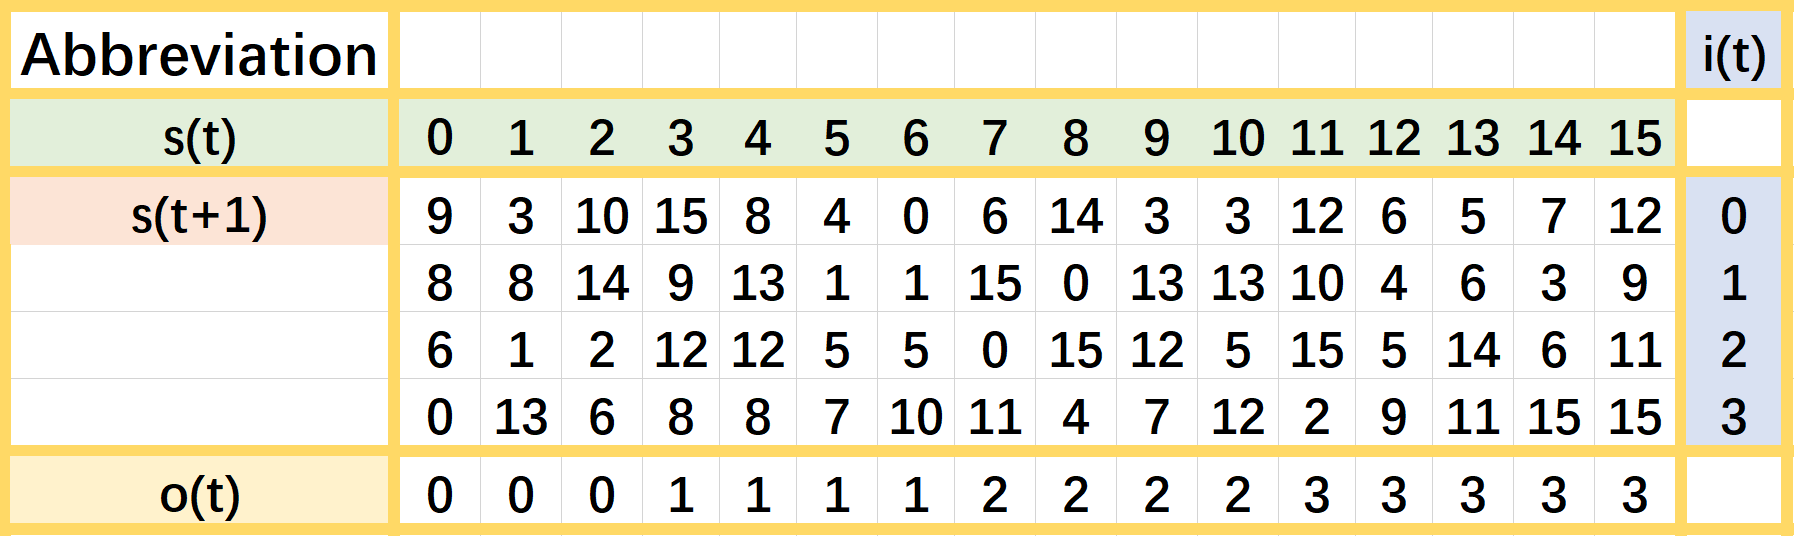
\includegraphics[scale=0.126]{figures/Fig7.png}}
	}}
      
      \caption{The algebraic form of the \BCN\ shown in Fig.\ref{fig:1}.}
      \label{fig:6}
   \end{figure}
   \label{exa:3}
\end{example}   


\subsection{Four existing observability of \BCNs}
After introducing the algebraic forms of \BCNs, we introduce four existing types of observability of \BCNs\ in this subsection. In order to introduce four existing types of observability of \BCNs, we define the mappings \cite{Zhang2016Observability}:
\begin{equation}
\begin{split}
L^k_{\mathsf{s}(0)} &: (\Delta_M)^k\mapsto(\Delta_N)^k,\ \mathsf{i}(0)\ldots \mathsf{i}({k-1}) \mapsto \mathsf{s}(1) \ldots\, \mathsf{s}(k)\\
L^{\infty}_{\mathsf{s}(0)} &: (\Delta_M)^{\infty}\mapsto(\Delta_N)^{\infty},\ \mathsf{i}(0) \mathsf{i}(1) \ldots  \mapsto \mathsf{s}(1) \mathsf{s}(2) \ldots
\end{split}
\label{equ:5}
\end{equation}
\begin{equation}
\begin{split}
(HL)^k_{\mathsf{s}(0)} &: (\Delta_M)^k\mapsto(\Delta_Q)^k,\ \mathsf{i}(0)\ldots \mathsf{i}(k-1) \mapsto \mathsf{o}(1)\ldots\, \mathsf{o}(k)\\
(HL)^{\infty}_{\mathsf{s}(0)} &: (\Delta_M)^{\infty}\mapsto(\Delta_Q)^{\infty},\ \mathsf{i}(0) \mathsf{i}(1) \ldots  \mapsto \mathsf{o}(1) \mathsf{o}(2)\ldots
\end{split}
\label{equ:6}
\end{equation}

Where $\Delta_N$, $\Delta_M$ and $\Delta_Q$ are three alphabets, $s_0\in \Delta_N$, $k\in \mathbb{Z}_+$ and $\infty$ is the infinite natural numbers. For all  $k\in \mathbb{N}^*$, 
\[\mathsf{I}=\mathsf{i}(0)\ldots \mathsf{i}({k-1}) \in(\Delta_M)^k\] 
is an input sequence, 
\[L^k_{\mathsf{s}(0)}(\mathsf{I})=\mathsf{s}(1) \ldots\, \mathsf{s}(k) \in(\Delta_N)^k\]
 is a state sequence, and 
 \[(HL)^k_{\mathsf{s}(0)}(\mathsf{I})=\mathsf{o}(1)\ldots\, \mathsf{o}(k) \in(\Delta_Q)^k\] 
 is a output sequence. For the $\infty$, 
 \[\mathsf{I}=\mathsf{i}(0) \mathsf{i}(1)\ldots  \in(\Delta_M)^{\infty}\] 
 is an infinitely long input sequence, 
 \[L^{\infty}_{\mathsf{s}(0)}(\mathsf{I})=\mathsf{s}(1) \mathsf{s}(2)\ldots  \in(\Delta_N)^{\infty}\] 
 is an infinitely long state sequence, and 
 \[(HL)^{\infty}_{\mathsf{s}(0)}(\mathsf{I})=\mathsf{o}(1) \mathsf{o}(2)\ldots \in(\Delta_Q)^{\infty}\]
  is an infinitely long output sequence. From the algebraic forms of \BCNs, in the formula (\ref{equ:5}), for any $1\le t \le |\mathsf{I}|$ we have 
 \[\mathsf{s}(t)=L\ltimes\mathsf{i}({t-1})\ltimes\mathsf{s}({t-1}).\] 
 In the formula (\ref{equ:5}) and formula (\ref{equ:6}), for any $1\le t \le |\mathsf{I}|$ we have  
 \[\mathsf{o}(t)=H\ltimes\mathsf{s}(t)=H\ltimes L\ltimes\mathsf{i}({t-1})\ltimes\mathsf{s}({t-1}).\] 

These mappings describe the relations of initial state ($\mathsf{s}(0)$), input sequence ($\mathsf{I}$), state sequence ($L^k_{\mathsf{s}(0)}(\mathsf{I})$ and $L^{\infty}_{\mathsf{s}(0)}(\mathsf{I})$) and output sequence ($(HL)^k_{\mathsf{s}(0)}(\mathsf{I})$ and $(HL)^{\infty}_{\mathsf{s}(0)}(\mathsf{I})$). Such that, four existing types of observability of BCNs can be defined as follows.
%And for all $1\ge k \ge j \ge |I|$, we use I[k,j] to denote the word $i_k \ldots i_j$ as an input sequence. 
\begin{definition} [First Observability]
The first type of observability is that, a \BCN\ is called observable, if for every initial state \State$^{i}(0)$$\in \Delta_N$, there exists an input sequence $\mathsf{I}\in(\Delta_M)^k$ for some $k\in \mathbb{N}^*$ such that for all states $\mathsf{s}^{i}(0)\neq \mathsf{s}^{j}(0)\in \Delta_N$, $H\ltimes\mathsf{s}^{i}(0)=H\ltimes\mathsf{s}^{j}(0)$ implies $(HL)^k_{\mathsf{s}^{i}(0)}(\mathsf{I})\neq (HL)^k_{{\mathsf{s}^{j}(0)}}(\mathsf{I})$ \cite{cheng2009controllability}.
\end{definition}

Hence the first observability means that if a \BCN\ is observable, then every initial state \State$^{i}(0)$ of the \BCN\ can be distinguished from other types of initial state by an input sequence $\mathsf{I}\in(\Delta_M)^k$. However, we can only use the corresponding input sequence $\mathsf{I}$ of an initial state $\mathsf{s}^{i}(0)$ to check whether the initial state $\mathsf{s}(0)$ of this \BCN\ is the state $\mathsf{s}^{i}(0)$.
\begin{example}
For example, for the \BCN\ mentioned in {\em Example \ref{exa:2}}, we have for every initial state of this \BCN\ can be distinguished from other types of initial state by an input sequence $\mathsf{I}\in(\Delta_M)^k$.  For instance,
\begin{itemize}
  \item the state $\delta_{16}^1$ can be determined by any input sequence which with the prefix $\delta_{4}^4$, $\delta_{4}^1  \delta_{4}^3$ or $\delta_{4}^1 \delta_{4}^4$, etc;
  \item the state $\delta_{16}^2$ can be determined by any input sequence which with the prefix $\delta_{4}^1$, $\delta_{4}^3$ or $\delta_{4}^4$, etc;
  \item the state $\delta_{16}^3$ can be determined by any input sequence which with the prefix $\delta_{4}^2$, $\delta_{4}^4$ or $\delta_{4}^1 \delta_{4}^4$, etc.
\end{itemize} 

Therefore we have this \BCN\ satisfies the existing first observability.
\label{exa:4}
\end{example}   

\begin{definition}[Second Observability]
	The second type of observability is that, a \BCN\ is called observable if for any distinct states $\mathsf{s}^{i}(0)$, $\mathsf{s}^{j}(0) \in \Delta_N$, there exists an input sequence $\mathsf{I}\in(\Delta_M)^k$ for some $k\in \mathbb{N}^*$, such that $H\ltimes\mathsf{s}^{i}(0)=H\ltimes\mathsf{s}^{j}(0)$ implies $(HL)^k_{\mathsf{s}^{i}(0)}(\mathsf{I})\neq (HL)^k_{\mathsf{s}^{j}(0)}(\mathsf{I})$ \cite{Zhao2010Input}.
\end{definition}

The second observability means that a \BCN\ is called observable if for every two distinct initial states $\mathsf{s}^{i}(0), \mathsf{s}^{j}(0)$ of the \BCN, there exists an input sequence $\mathsf{I}\in(\Delta_M)^k$ which can distinguish them. 
\begin{example}
For example, for the \BCN\ mentioned in {\em Example \ref{exa:2}}, we have for every two distinct initial states of the \BCN, there exists an input sequence $\mathsf{I}\in(\Delta_M)^k$ which can distinguish them.  For instance,
\begin{itemize}
  \item the states $\delta_{16}^1$ and $\delta_{16}^2$ can be distinguished by any input sequence which with the prefix $\delta_{4}^1$, $\delta_{4}^2 \delta_{4}^1$ or $\delta_{4}^2 \delta_{4}^2$, etc;
  \item the states $\delta_{16}^1$ and $\delta_{16}^3$  can be distinguished by any input sequence which with the prefix $\delta_{4}^2$, $\delta_{4}^3$ or $\delta_{4}^4$, etc;
  \item the states $\delta_{16}^2$ and $\delta_{16}^3$  can be distinguished by any input sequence which with the prefix $\delta_{4}^1$, $\delta_{4}^2$ or $\delta_{4}^4$, etc.
\end{itemize} 

Therefore we have this \BCN\ satisfies the existing second observability.
\label{exa:5}
\end{example}   
\begin{definition}[Third Observability]
The third type of observability is that, a \BCN\ is called observable if there exists an input sequence $\mathsf{I}\in(\Delta_M)^k$ for some $k\in \mathbb{N}^*$, such that for any distinct states $\mathsf{s}^{i}(0)$, $\mathsf{s}^{j}(0) \in \Delta_N$, $H\ltimes\mathsf{s}^{i}(0)=H\ltimes\mathsf{s}^{j}(0)$ implies $(HL)^k_{\mathsf{s}^{i}(0)}(\mathsf{I})\neq (HL)^k_{\mathsf{s}^{j}(0)}(\mathsf{I})$ \cite{Cheng2011Identification}.
\end{definition}

The third observability means that a \BCN\ is called observable if there exists an input sequence $\mathsf{I}\in(\Delta_M)^k$ which can determine the initial state $\mathsf{s}(0)$ of the \BCN\ for every $\mathsf{s}(0)\in\Delta_N$.

\begin{example}
For example, for the \BCN\ mentioned in {\em Example \ref{exa:2}}, we have there is an input sequence $\mathsf{I}\in(\Delta_M)^k$ which can determine the initial state of this \BCN. For instance, any input sequence which with the prefix $\delta_{4}^1\delta_{4}^4\delta_{4}^1$ can determine the initial state $\mathsf{s}(0)$ of the \BCN\ for every $\mathsf{s}(0)\in\Delta_N$.

Therefore we have this \BCN\ satisfies the existing third observability.
\label{exa:6}
\end{example}  
\begin{definition}[Fourth Observability]
	The fourth type of observability is that, \BCN\ is called observable, if for any input sequence $\mathsf{I}\in(\Delta_M)^{\infty}$, for any distinct states $\mathsf{s}^{i}(0)$, $\mathsf{s}^{j}(0) \in \Delta_N$, $H\ltimes\mathsf{s}^{i}(0)=H\ltimes\mathsf{s}^{j}(0)$ implies $(HL)^{\infty}_{\mathsf{s}^{i}(0)}(\mathsf{I})\neq (HL)^{\infty}_{\mathsf{s}^{j}(0)}(\mathsf{I})$ \cite{Fornasini2013Observability}.
\end{definition}

The fourth observability means that a \BCN\ is called observable if every sufficient long input sequence $\mathsf{I}\in(\Delta_M)^{\infty}$ can determine the initial state $\mathsf{s}(0)$ of the \BCN\ for every $\mathsf{s}(0)\in\Delta_N$.
\begin{example}
For example, for the \BCN\ mentioned in {\em Example \ref{exa:2}}, we have there exists at least one sufficient long input sequence that can not determine the initial state of this \BCN. For instance, the states $\delta_{16}^4$ and $\delta_{16}^5$  will convert into $\delta_{16}^{13}$ after being affected by $\delta_{4}^3$, therefore any input sequence which with the prefix $\delta_{4}^3$, they can not determine the initial state $\mathsf{s}(0)$ of the \BCN\ for every $\mathsf{s}(0)\in\Delta_N$.

Therefore we have this \BCN\ does not satisfy the existing fourth observability.
\label{exa:7}
\end{example}  

What is more, we know the implication relationships of four existing types of observability from the definitions of them shown in Fig.\ref{fig:9} \cite{Zhang2016Observability}. 

 \begin{figure}[thpb]
      \centering
      \framebox{\parbox{3in}{
		\centerline{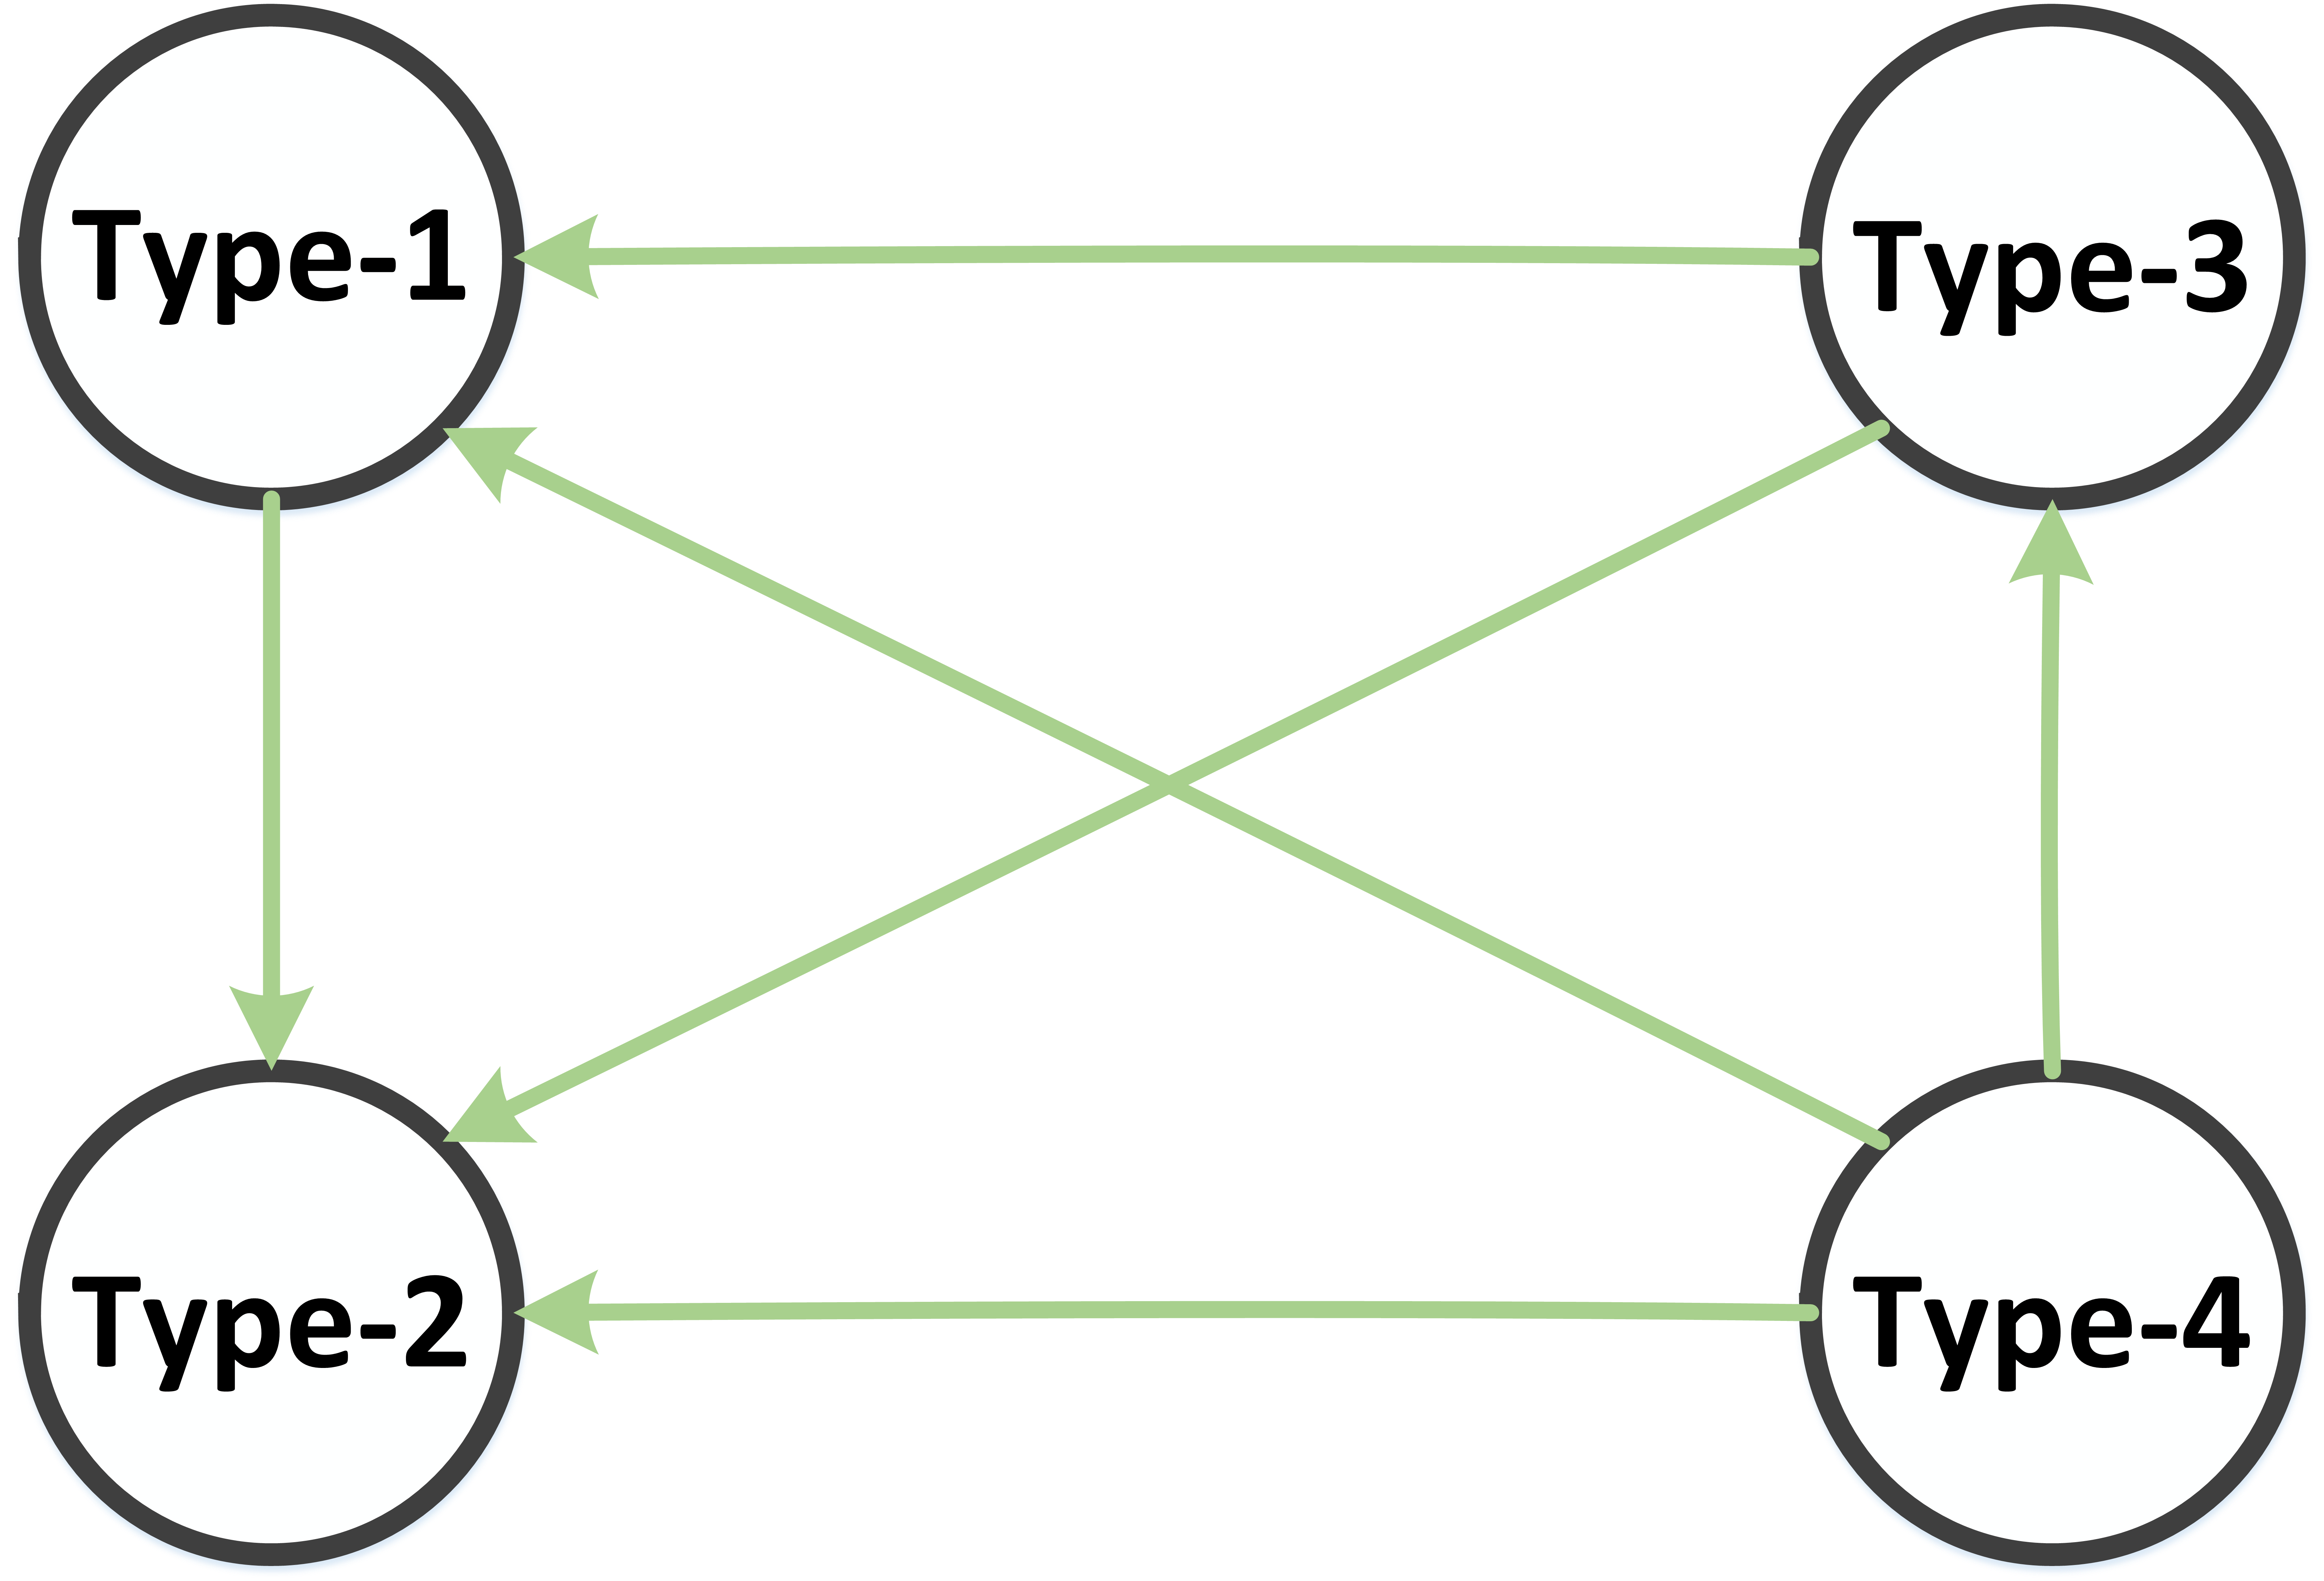
\includegraphics[scale=0.27]{figures/Fig9.png}}
	}}
      
      \caption{The implication relationships graph between existing observability 1, 2, 3, 4, where ``$\rightarrow$" means ``implies".}
      \label{fig:9}
   \end{figure}
%\begin{proposition}
%The implication relationships of four existing types of observability.
%\begin{itemize}
%\item The first observability implies the second observability, but the second observability does not imply the first observability.\\
%\item The third observability implies the second observability, but the second observability does not imply the third observability.\\
%\item The third observability implies the first observability, but the first observability does not imply the third observability.\\
%\item The fourth observability implies the third observability, but the third observability does not imply the fourth observability.\\
%\item The fourth observability implies the second observability, but the second observability does not imply the fourth observability.\\
%\item The fourth observability implies the first observability, but the first observability does not imply the fourth observability. \\
%\end{itemize} 
%\end{proposition}

Where the implication relationship is that ``The first observability implies the second observability.'' means ``If a \BCN\ satisfies the first observability, then it satisfies the second observability.'' For the details of the proving process of this proposition, we refer readers to \cite{Zhang2016Observability}.
%, when we don't presuppose the initial state of {\em BCNs}
   
After introducing the definition of four existing observability and their implication relationship, we discuss how to determine the initial state of some \BCNs\ by four existing types of observability. 
\begin{itemize}
\item The first and second observability can not help us to determine the initial state of some \BCNs. Because in the first observability, firstly, we need to assume that the initial state $\mathsf{s}(0)$ of a \BCN\ is $\mathsf{s}^{i}(0)$. Secondly, we check it by corresponding input sequence $\mathsf{I}$ of $\mathsf{s}^{i}(0)$. If $\mathsf{s}(0)=\mathsf{s}^{i}(0)$, then we can determine the initial state. But if $\mathsf{s}(0)\ne \mathsf{s}^{i}(0)$, then we can not determine the initial state of the \BCN. Therefore we need to repeat this determining procedure untill we can determine the initial state. %check several test cases (which with the same initial state $\mathsf{s}(0)$) of this \BCN\  of them. 
So do the existing second observability of \BCNs.
\item We can use the third existing observability and fourth existing observability to determine the initial state $\mathsf{s}(0)$ of \BCNs. But the requirements for \BCNs\ are very difficult to meet when we use the third observability and fourth observability. Because we do not make full use of the output and input in the process of determining the initial state. As the output of \BCNs\ we observed at every time step can help us further determine the range of the initial state. We can use different input sequence to determine the initial state based on the range of the initial state. But in the third and fourth existing observability, we use the same input sequence to determine the initial state.
\end{itemize} 
 
In some biological systems (depicted by \BCNs), the initial state of them can be checked at most once. Therefore, we can not use the first observability and second observability to determine the initial states of them. Moreover, in some biological systems, it would takes many costs to check these biological systems. Hence it would cost a lot of overhead for us to determine the initial state of them by the first observability and second observability. Furthermore, we can not use the third observability and fourth observability to determine the initial states of some biological systems if they do not satify the requirements of the third and fourth observability. With these disadvantages of four existing observability, we propose the online observability of \BCNs\ to solve this problem.

 \begin{problem}
\label{pro:2}
What is the necessary and sufficient condition of determine the initial state $\mathsf{s}(0)$ of the \BCN\ for every $\mathsf{s}(0)\in\Delta_N$?
\end{problem}